






                      %%% RELATIONS %%%
\chapter {Relations}
Relations support comparisons or connections between elements within a set or between two or more sets, or between members of the same set. For example ``less than or equal'', ``is perpendicular to'', ``is a cousin to'' are relations on a set of numbers, lines, or people. 

Relations are closely associated with functions but we looked at those first since you are familiar with them from before. Relations are a superset of functions, all functions are relations but not all relations are functions.

The fundamental restriction to a function is that it needed to evaluate to exactly one value. A relation can be a many-to-many mapping from the domain to the codomain. In its most abstract statement, all valid subsets of the cross product of the domain and codomain are relations.

A fundamental paradigm is one called objects/relations and is found in programming languages today. We saw that sets are collections of objects and we saw that predicates take on the value true when a particular property is found in that object. Objects can have relationships among them and the most basic is the binary relationship. In a binary relationship we way that the two objects either are in or not in that relationship with each other. This chapter explores the consequences of this and its many applications.



\section {Relations}
\begin {definition}[Binary Relations]\index{binary relations}
Let $A$ and $B$ be sets. A \textit {binary relation $\mathrel{R}$ between $A$ and $B$} is a subset of the Cartesian Product $A \times B$. We can denote the binary relation on two elements $a$ and $b$ by $a\mathrel{R}b$, or by $(a,b)\in \mathrel{R}$. We can denote the lack of relationship $\mathrel{R}$ between the two elements with the notation $a\not\mathrel{R}b$ or $(a,b) \not \in R$. The sets $A$ and $B$ may be the same set in which case we say $\mathrel{R}$ is a relation on $A^2$ or on the set $A$. We read ``a is in relation to b'' or ``a is related to b'' to indicate they are related. \\

Relations are not limited to relations on two sets but can be applied to any number of sets. The relation is still defined as a subset of the n-tuples formed from the cross product of the sets.

Relations are sets of tuples of the cross product and set operators can be used on them.

Given a set $A$, the relation $\{(a,a)|a\in A\}$ is the equality or identity relation and is denoted by $\Delta_A$.
\end {definition} 

Note that functions are a subset of relations. Note that plotting graphs of functions uses the Cartesian plane which is a relation of $\mathbb{R}^2$. 

\subsection{Inverse Relation}
The \textit{inverse of a relation} $\mathrel{R}$ from set $A$ to $B$ is the relation denoted by $R^{-1} = \{(b,a)|(a,b)\in \mathrel{R}\}$.

    \subsection {Relational operators}
    Equality, inequality, greater than, greater than or equal, less than, less than or equals are all relational operators that every programmer learns. To these we introduce one that is not often seen in programming, the divides relation.
    
    \begin{definition}[Divides]\index{divides}
    If $a$ and $b$ are integers with $a\ne 0$, we say that \textit{$a$ divides $b$} if there is an integer $c$ such that $b = ac$, or equivalently $\frac{b}{a}$ is an integer. When $a$ divides $b$ we say that $a$ is a factor or divisor of $b$, and that $b$ is a multiple of $a$. The notation $a \mid b$ denotes that $a$ divides $b$. We write $a\nmid b$
when $a$ does not divide $b$.
    \end{definition}


\section {Properties of Relations}
    \begin {definition}[reflexive relation]\index{reflexive relation}
    A relation $R$ on a set $A$ is called \textit{reflexive} if $(a,a) \in R$ for every element $a \in A$. The relation $R$ is reflexive if $\forall a((a,a) \in R)$.
    \end {definition}
    
    \begin {definition}[Symmetric Relation]\index{symmetric relation}
    A relation $R$ on a set $A$ is alled \textit{symmetric} if $(b,a) \in R$ for all $a,b \in A$.
    \end {definition} 
    
    \begin {definition}[Antisymmetric]\index{antisymmetric}
    A relation $R$ on set $A$ such that for all $a,b \in A$, if $(a,b) \in R$ and $(b,a) \in R$, then $a=b$ is called \textit{antisymmetric}
    \end {definition}
    
    \begin {definition}
    A relation $R$ on a set $A$ is called \textit{transitive} if whenever $(a,b)\in R$ and $(b,c) \in R$, then $(a,c) \in R$. The relation $R$ on a set $A$ is transitive if we have $\forall a \forall b \forall c (((a,b) \in R \land (b,c) \in R) \rightarrow (a,c) \in R)$
    \end {definition}
    
    \begin{definition}[Anti-Reflexive Relation]\index{anti-reflexive relation}
    \end{definition}


\section {Composition of Relations}
Combining Relations in Rosen

\begin{definition}[Composition of Relations]\index{composition of relations}
Let $R$ be a relation from set $A$ to set $B$ and $S$ a relation from $B$ to a set $C$. The \textit{composite} of $R$ and $S$ is the relation consisting of ordered pairs $(a,c)$ such that $(a,b) \in R$ and $(b,c) \in S$. We denote the composite of $R$ and $S$ by $S \circ R$.
\begin{notes}
Carefully note the order of the operand in the composition operation.
\end{notes}
\end{definition}


\section {Graphic Representation of Relations}
For relations onto themselves, this gives what we will later call a directed graph. We cover graphs more formally in a later chapter.
    \subsection {Digraphs}
    A convenient pictorial representation of relations is to represent the domain and co-domain as ovals with the elements labeled. A pair that is in the relation is then represented by an arc from the element in the domain to the element in the co-domain. When the co-domain is the same as the domain the oval is sometimes omitted. We call this a \textit{directed graph}. We will cover directed graphs more formally in the chapter on Graphs.  

\section {Closure Property of Relations}
   \subsection {Transitive Closure of Relations}
   
   \begin{definition}
   Let $R$ be a relation on a set $A$. The \textit{connectivity relation $R^*$} consists of the pairs $(a,b)$ such that there is a path of length one from $a$ to $b$ in $R$.
   \end{definition}
   \subsection {Kleene Closure and Order}

\section {N-ary Relations}
We have only spoken of binary relations up to now. But more than two elements can be in a relation. 
\begin{definition}
Let $A_1,A_2, \dots ,A_n$ be sets. An \textit{n-ary relation} on these sets is a subset of $A_1 \times A_2 \times \dots \times A_n$. The sets $A_1,A_2, \dots ,A_n$ are called the \textit{domains} of the relation, and $n$ is called its \textit{degree}.
\end{definition}

\begin{definition}
Let $R$ be an $n$-ary relation and $C$ a condition that elements in $R$ may satisfy. Then the \textit{selection operator $s_C$} maps the $n$-ary relation $R$ to the $n$-ary relation of all $n$-tuples from $R$ that satisfy the condition $C$.
\end{definition}

\begin{definition}
The \textit{projection} $P_{i_1i_2, \dots ,i_m}$ where $i_1 < i_2 < \dots i_m$, maps the $n$-tuple ($a_1,a_2, \dots , a_n$) to the $m$-tuple ($a_{i_1},a_{i_2}, \dots ,a_{i_m}$), where $m \le n$.
\end{definition}

    \subsection {Application to Databases}

\section {Matrices and Linear Algebra}
Many include matrices in Discrete Mathematics. We exclude this since it is offered as a separate course.











\section{Representations of Relations}
The definition of relations are as a subset of the cross product $A \times B$. But two alternate representations of relations are useful.
  \subsection{Representing Relations Using Matrices}
  Given a subset of $A \times B$, one can represent the relation by creating a matrix with the elements of the sets $A$ and $B$ along the two axes of the matrix and entering a 1 when that pair is in the relation and 0 if not. 
  
  
  
  \subsection{Representing Relations Using Digraphs}
  \subsection{Paths in Directed Graphs}

\section{Closures on Relations}
  \subsection{Closures}
Sometimes an operation will return something that is outside the set from which the argument was drawn. For example, you can perform division on two integers but not get an integer as a return value. You can solve an equation like $2\cdot 2x+1=0$ with 2 and 1 both being valid rational numbers yet find you have a number that is outside the set of rational numbers. We say that the set is not closed under these operation                                  s. 

When we look at the properties of relations sometimes we see that a given relation is closed, that is every pair needed to satisfy that relation are found in the relation. When we find that to be true, we say the set is closed under that relation.

Let $R$ be a relation on a set $A$. $R$ may or may not have some property \textbf{P}, say reflexivity. If the set $A$ does not possess the property, it is possible to add pairs to the relation such that the union of the two relations (which after all are just sets of pairs) will possess that property. We are now ready to offer a formal definition.

\begin{definition}[Closure]\index{closure}
A set that is closed under an operation or collection of operations is said to satisfy a closure property. When a set $S$ is not closed under some operations, one can usually find the smallest set containing $S$ that is closed. This smallest closed set is called the closure of $S$ (with respect to these operations). For example, the closure under subtraction of the set of natural numbers, viewed as a subset of the real numbers, is the set of integers. The closure of a set $S$ which does not posses the closure property under the reflexion relation can be created by summing the relation with all pairs that make the relation reflexive.
\end{definition}
The reflexive closure of a relation$R$can be formed by adding to $R$ all pairs of the form $(a,a)$with$a\in A$,not already in$R$. The addition of these pairs produces a new relation that is reflexive, contains$R$,and is contained within any reflexive relation containing $R$. We see that the reflexive closure of $R$ equals $R \cup \Delta$, where $\Delta=\{(a,a)\vert a\in A\}$is the diagonal relation on$A$.
 
  \subsection{Transitive Closures}

\begin{definition}
Let $R$ be a relation on a set $A$. The \textit{connectivity relation $R^*$} consists of the pairs $(a,b)$ such that there is a path of length at least one from $a$ to $b$ in $R$.
\end{definition}

\begin{theorem}
The transitive closure of a relation $R$ equals the connectivity relation $R^*$.
\end{theorem}

\begin{lemma}
Let $A$ be a set with $n$ elements, and let $R$ be a relation on $A$. If there is a path of length at least one in $R$ from $a$ to $b$, then there is such a path with length not exceeding $n$. Moreover, when $a \ne b$, if there is a path of length at lteast one from $R$ from $a$ to $b$, then there is such a path with length not exceeding $n-1$.
\end{lemma}

  \subsection{Computing Transitive Closures} 
  The most well known algorithm to compute the transitive closure of a relation is Warshall's Algorithm.

 
\section {Equivalence Relations}
reflective, symmetric, transitive
remainder function partitions

    \subsection {Equivalence Classes and Set Partitions}

\begin{definition}
The elements $a$ and $b$ that are related by an equivalence relatin are called \textit{equivalent}. The notation $a \sim b$ is often used to denote that $a$ and $b$ are equivalent elements with respect to a particular equivalence relation.
\end{definition}

\begin{definition}
Let $R$ be an equivalence relation on a set $A$. The set of all elements that are related to an element $a$ of $A$ is called the \textit{equivalence class} of $a$. The equivalence class of $a$ with respect to $R$ is denoted by $[a]_R$. When only one relation is under consideration, we can delete the subscript $R$ and write $[a]$ for this equivalence class.

If $b \in [a]_R$, then $b$ is called a \textbf{representative} of this equivalence class.
\end{definition}


\begin{theorem}
Let $R$ be an equivalence relation on a set $A$. These statements for elements $a$ and $b$ of $A$ are equivalent:
\begin{enumerate}[label=(\roman*)]
\item
$aRb$
\item
$[a]=[b]$
\item
$[a] \cap [b] \neq \emptyset$
\end{enumerate}
\end{theorem}

\begin{theorem}
Let $R$ be an equivalence relation on a set $S$. Then the equivalence classes of $R$ form a partition of $S$. Conversely, given a partition $\{A_i | i \in I\}$ of the set $S$, there is an equivalence relation $R$ that has the sets $A_i, i \in I$, as its equivalnece classes.
\end{theorem}

    \subsection {Partial Ordering Relations}
\begin{definition}[Posets]\index{poset}\index{partial order}
A relation $R$ on a set $S$ is called a \textit{partial ordering} or \textit{partial order} if it is reflexive, antisymemetric, and transitive. A set $S$ together with a partial ordering $R$ is called a \textit{partially ordered set} or \textit{poset}, denoted by $(S,R)$. Members of $S$ are called \textit{elements} of the poset.
\end{definition}

Many different relations on sets create posets such as $\ge$, evenly divides (|), and $\subset$. We create a new relation symbol $\preceq$.

\begin{definition}
Given a poset $(S,R)$ and two elements $a$, $b$, we use the notation $a \preceq b$ to indicate that $(a,b)\in R$. We use $\preceq$ to designate any relation of a poset. The elements $a$ and $b$ of a poset $(S,\preceq)$ are called \textit{comparable} if either $a\preceq b$ or $b\preceq a$. When $a$ and $b$ are selements of $S$ such that neither $a \preceq b$ nor $b \preceq a$, $a$ and $b$ are called \textit{incomparable}. If $a \preceq b$ and $a \neq b$, we use the notation $a \prec b$.
\end{definition}

\begin{notes}
Object oriented programming languages allow you to code relations. Note that since two elements of a set may be incomparable given the relation $\preceq$, we call it a partial ordering.
\end{notes}
    
\begin{definition}
If $(S,\preceq)$ is a poset and every two elements of $S$ are comparable, $S$ is called a \textit{totally ordered} or \textit{linearly ordered set}, and $\preceq$ is called a \textit{total order} or a \textit{linear order}. A totally ordered set is also called a \textit{chain}.
\end{definition}

\begin{definition}[Well-Ordered Set]\index{well-ordered set}
The poset $(S,\preceq)$ is called a \textit{well-ordered set} if it is a poset such that $\preceq$ is a total ordering and every nonempty subset of $S$ has a least element, (something defined in a few sections).
\end{definition}

\begin{theorem} [The Principle of Well-Ordered Induction]
Suppose that $S$ is a well-ordered set. Then $P(x)$ is true for all $x \in S$, if
INDUCTIVE STEP: For every $y\in S$, if $P(x)$ is true for all $x\in S$ with $x \prec y$, then $P(y)$ is true.
\begin{proof}
Suppose it is not the case that $P(x)$ is true for all $x\in S$. Then there is an element $y\in S$ such that $P(y)$ is false. Consequently, the set $A=\{x\in S | P(x) is false \}$ is nonempty. Because $S$ is well ordered, $A$ has a least element $a$. By the choice of $a$ as a least element of $A$, we know that $P(x)$ is true for all $x\in S$ with $x\prec a$. This implies by the inductive step $P(a)$ is true. This contradiction shows that $P(x)$ must be true for all $x\in S$.
\end{proof}
\begin{notes}
We do not need a basis step in a proof using the principle of well-ordered induction because if $x_0$ is th eleast element of a well ordered set, the inductive step tells us that $P(x_0)$ is true. This follows because there are no elements $x\in S$ with $x\prec x_0$.
\end{notes}
\end{theorem}


    \subsection {Lexicographic Order}\index{lexicographic order}
You may have already noticed that the way words get arranged in a dictionary are different than the way they would be sorted if they were numbers. This ordering of strings is called a lexicographic ordering. Consider two posets $(A_1,\preceq_1)$ and $(A_2,\preceq_2)$. The \textbf{lexicographic ordering} $\preceq$ on $A_1 \times A_2$ is defined by specifing how one pair, $(a_1,a_2)$ is less than another $(b_1,b_2)$. We say $(a_1,a_2) \prec (b_1,b_2)$ if either $a_1 \prec_1 b_1$ or if both $a_1= b_1$ and $a_2 \prec b_2$.

\begin{notes}
This came from Rosen. why are there two different relationships in this presentation?
\end{notes} 

\begin{definition}[Lexicographic Ordering]
Given strings $a_1a_2 \dots a_m$ and $b_1b_2 \dots b_n$ on a partially ordered set $s$. Suppose these strings are not equal. Let $t$ minimim of  $m$ and $n$. We define the string $A$ as less than $B$ if and only if
$$(a_1,a_2, \dots ,a_t) \prec (b_1,b_2, \dots ,b_t),$$
or
$$(a_1,a_2, \dots ,a_t) = (b_1,b_2, \dots ,b_t) \land m<n$$
\end{definition}

    \subsection {Haase Diagrams}\index{Haase diagram}
Consider Figure 9-6-3a of a small poset $(\{1,2,3,4,6,8,12\}, |)$. This Recall that a poset is a partial ordering and that means it is reflexive, anti-symmetric and transitive. If we know that the di-graph is of a poset we can then remove the reflexive edges. This gives us Figure 9-6-3b which has the reflexive edges removed. Since we know it must also be transitive we can safely remove those edges as well. If we use the convention that vertices that are "less than" in the ordering be placed lower on the graph we can also remove the directed edges and replace them with undirected edges. This gives Figure 9-6-3c which is known as a Haase Diagram or ordering diagram and represents the poset in an economical visual fashion.

   \begin{table}[htbp]
   \centering
   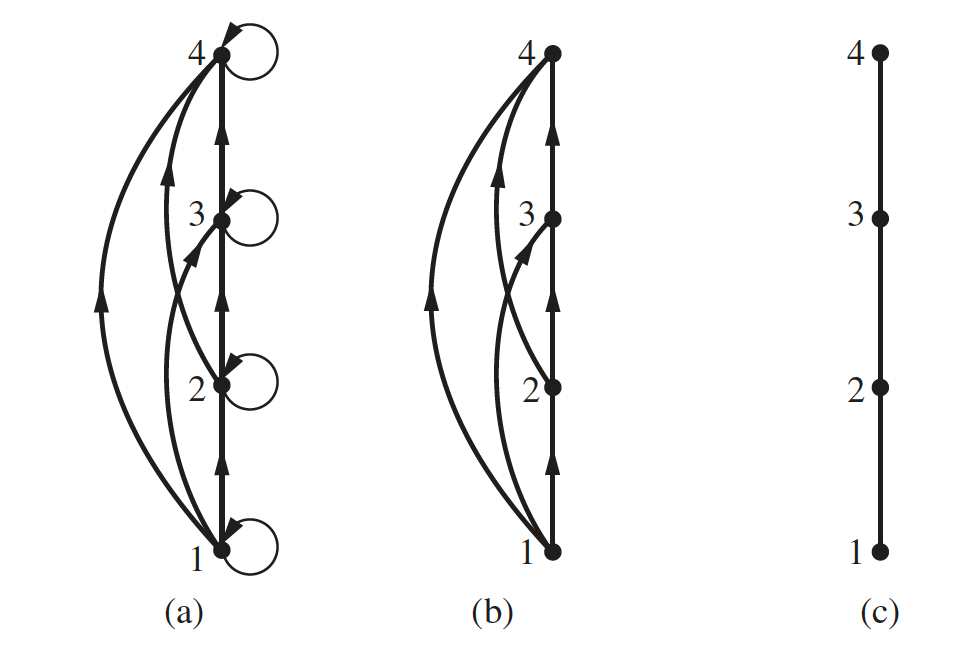
\includegraphics [width=3in]{Figure-9-6-2-ConstructionOfHaaseDiagram}
   \caption{Construction of a Hasse Diagram }
   \label{figure:Construction of a Hasse Diagram }
   \end{table}


    \subsection {Maximal and Minimal Elements}
When discussing the basic axioms of arithmetic that a student can assume in proofs, we introduced the Completeness Property (Definition \ref{CompletenessProperty}). We now add to that.

Posets have properties that are useful to some applications, in particular maximal and minimal elements. 

\begin{definition}[Upper and Lower Bounds]
An element of  a poset is called maximal if it is not less than any element o f the poset. That is, $a$ is \textbf{maximal} in the poset $(S,\preceq)$ if there is no $b\in S$ such that $a \prec b$. Similarly, an element of a poset is called minimal if it is not greater than any element of the poset. That is, $a$ is \textbf{minimal} if there is no element $b\in S$ such that $b \prec a$. Maximal and minimal elements are the top and bottom elements in a Haase Diagram.

If an element $a$ is called the \textbf{greatest element} of the poset $S$ if $b\preceq a$ for all $b \in S$. The greatest element is unique when it exists. Likewise, an element is called the least element if it is less than all the other elements in the poset. The element $a$ of a poset is the \textbf{least element} of $(S,\preceq)$ if $a\preceq b$ for all $b\in S$. The least element is unique when it exists.
\end{definition}

\begin{definition}[Least Upper Bound]\index{least upper bound}
The element $x$ is called the \textbf{least upper bound} of the subset $A$ if $x$ is an upper bound that is less than every other upper bound of $A$. Because there is onlyu one such element, if it exists, it makes sense to call this element \textit{the} least upper bound. That is, $x$ is the least upper boundf of $A$ if $a\preceq x$ whenever $a \in A$, and $x \preceq z$ whenever $z$ is an upper bound of $A$. Similarly, the ...
We denote these as glb($A$) and lub($A$). 
\end{definition}

\subsection{Lattices}
\begin{definition}[Lattice]\index{lattice}
A partially ordered set in which every pair of elements has both a least upper bound and a greatest lower bound is called a \textbf{lattice}.
\end{definition}

    \subsection {Topological Sorting}
\begin{definition}[Topological Sort]\index{topological sort}
A total ordering $\preceq$ is said to be \textbf{compatible} with the partial ordering $R$ if $a \preceq b$ whenever $aRb$. Constructing a compatible total ordering from a partial ordering is called \textbf{topological sorting} or as some mathematicians will say, a linearization of a partial ordering.
\end{definition}

\begin{lemma}\label{ExistenceOfMinimalElementInAPoset}
Every finite nonempty poset $(S,\preceq)$ has at least one minimal element.
\end{lemma}



\section{$n$-ary Relations and Their Applicaiton for Databases}
An innovation of database technology was the application of relations.

\begin{definition}
Let $A_1,A_2,\ldots,A_n$ be sets and an $n$-ary relation on these sets as a subset of $A_1\times A_2\times \ldots \times A_n$. The sets $A_1,A_2, \ldots, A_n$ are called the domains of the relation, and $n$ is called its \textit{degree}.
\end{definition}

Let the terms of the $n$-tuple represent datafields. Then each domain is a set of values that the datafield can take on. Each tuple in the relation can be treated like a record in a data processing system and the collection of them can be presented in a table where each column represents each of the elements drawn from the domains. By putting them into an $n$-tuple, we establish a relationship among those elements. We call this part of a relational data model. 

Often the fields have a functional relation to one or more other elements. That is, given the key field, the other element in the domain is uniquely determined. When such a functional relationship exists from one of the domains to another, we say the pre-image is the key to the table. If this holds for all the terms in the tuple we call this field the primary key for the table. 

We define an operation on a table called selection:
\begin{definition}
Let $\mathrel{R}$ be an $n$-ary relation and $C$ a predicate that elements of $\mathrel{R}$ may satisfy. Then the selection operator $s_c$ maps the $n$-ary relation $\mathrel{R}$ to the $n$-ary relation from $\mathrel{R}$ of all $n$-tuples from $\mathrel{R}$ that satisfy the predicate C.
\end{definition}
 
\newpage


